%%%%%%%%%%%%%%%%%%%%%%%%%%%%%%%%%%%%%%%%%
% St Sectioned Assignment
% LaTeX Template
% Version 1.0 (5/5/12)
%
% This template has been downloaded from:
% http://www.LaTeXTemplates.com
%
% Original author:
% Frits Wenneker (http://www.howtotex.com)
%
% License:
% CC BY-NC-SA 3.0 (http://creativecommons.org/licenses/by-nc-sa/3.0/)
%
%%%%%%%%%%%%%%%%%%%%%%%%%%%%%%%%%%%%%%%%%

%----------------------------------------------------------------------------------------
%	PACKAGES AND OTHER DOCUMENT CONFIGURATIONS
%----------------------------------------------------------------------------------------

\documentclass[paper=a4, fontsize=11pt]{scrartcl} % A4 paper and 11pt font size

\usepackage[T1]{fontenc} % Use 8-bit encoding that has 256 glyphs
%\usepackage{fourier} % Use the Adobe Utopia font for the document - comment this line to return to the LaTeX default
\usepackage[english]{babel} % English language/hyphenation
\usepackage{amsmath,amsfonts,amsthm} % Math packages

\usepackage{lipsum} % Used for inserting dummy 'Lorem ipsum' text into the template
\usepackage{graphicx}

\usepackage{sectsty} % Allows customizing section commands
\allsectionsfont{\centering \normalfont\scshape} % Make all sections centered, the default font and small caps

\usepackage{hyperref}


\usepackage{fancyhdr} % Custom headers and footers
\pagestyle{fancyplain} % Makes all pages in the document conform to the custom headers and footers
\renewcommand{\headrulewidth}{0pt} % Remove header underlines
\renewcommand{\footrulewidth}{0pt} % Remove footer underlines
\setlength{\headheight}{13.6pt} % Customize the height of the header

\numberwithin{equation}{section} % Number equations within sections (i.e. 1.1, 1.2, 2.1, 2.2 instead of 1, 2, 3, 4)
\numberwithin{figure}{section} % Number figures within sections (i.e. 1.1, 1.2, 2.1, 2.2 instead of 1, 2, 3, 4)
\numberwithin{table}{section} % Number tables within sections (i.e. 1.1, 1.2, 2.1, 2.2 instead of 1, 2, 3, 4)

\setlength\parindent{0pt} % Removes all indentation from paragraphs - comment this line for an assignment with lots of text

%----------------------------------------------------------------------------------------
%	TITLE SECTION
%----------------------------------------------------------------------------------------

\newcommand{\horrule}[1]{\rule{\linewidth}{#1}} % Create horizontal rule command with 1 argument of height



\renewcommand{\vec}[1]{\textbf{#1}}
\newcommand{\ssvec}[1]{\textsf{\textbf{#1}}}

\newcommand{\veca}{\vec{a}}
\newcommand{\vecx}{\vec{x}}
\newcommand{\vecy}{\vec{y}}
\newcommand{\vecz}{\vec{z}}

\newcommand{\rveca}{\ssvec{a}}
\newcommand{\rvecx}{\ssvec{x}}
\newcommand{\rvecy}{\ssvec{y}}
\newcommand{\rvecz}{\ssvec{z}}

\newcommand{\yone}{\textsf{y}_1}
\newcommand{\ytwo}{\textsf{y}_2}

\newcommand*{\everymodeprime}{\ensuremath{\prime}}

\begin{document}


%----------------------------------------------------------------------------------------
%	PROBLEM 1
%----------------------------------------------------------------------------------------
\newpage

NOTE: the goal is to be headed in right direction for research, and also have some subset/version be implementable before June 15 (Nick's Roy's deadline) \\

This is meant as a first complete description and there are many opportunities for improving and increasing complexity, including model complexity and including a Bayesian update for control decisions as another way to include hysteresis.\\  

%\horrule{1pt} 
%\\


\textbf{Assumptions of problem}
\\

Our actual hardware system is a quadrotor UAV with all onboard sensing and computation, and most relevant parameters of this system are: 
\begin{itemize}
\item Up to 15 m/s velocity towards obstacles
\item At full speed, expected stopping distance is in the range of 20+ m
\item A 5 m range, 120 x 160 depth image is available at 30 Hz
\item Estimates for x, y, z linear velocities and covariances are available at 30 Hz
\item Due to the difficulty of state estimation at high speeds, the uncertainty for the velocity estimates are expected to be high: perhaps as high as +/- 5 m/s for 1-$\sigma$.  (Note that even though a graph-based state estimation is used (iSAM), internally the state estimator linearizes the graph to use a Gauss-Newton solver, and so Gaussian covariances are straightforward to provide.)
\item A higher level system provides the ``global navigation function'' which evaluates $cost(\mathbb{A}_i)_{\text{towards goal}} $ for us.
\item An inner-loop attitude controller will stabilize desired attitude and thrust setpoints at 200+ Hz with the IMU alone for attitude estimation. (This is very practical, due to high IMU rates and sufficiency for estimating attitudes.)
\end{itemize}

Note that at maximum speed, the stopping distance is larger than the range of the depth sensing information.  Hence the primary goal is, to the best of the quadrotor's noisy information, swerve to avoid obstacles. \textit{At full speed, stopping for safety is not an option. Swerving towards the most dynamically feasible open area is the only option}.  At speeds low enough such that the stopping distance is less than the sensing horizon, however, we also want a system that will naturally choose stopping. \\

An assumption we make at least in this initial approach is that the quadrotor plant in feedback with the inner-loop attitude controller can be approximated by a simple double integrator model with drag.  Although this does not capture the attitude dynamics of the vehicle (it takes time for the vehicle to switch from a roll-right to a roll-left), the attitude dynamics of the vehicle are much faster than the velocity dynamics.  There are advantages for us starting with this simple linear model with Gaussian noise, that has independence of $x, y,$ and $z$ (both for computational complexity, and for reasoning about), and it is my guess that this simple model can be taken far before its limits are shown. It is, however, an approximation that is inherent to the simplicity of a quadrotor.\\

\begin{figure}
  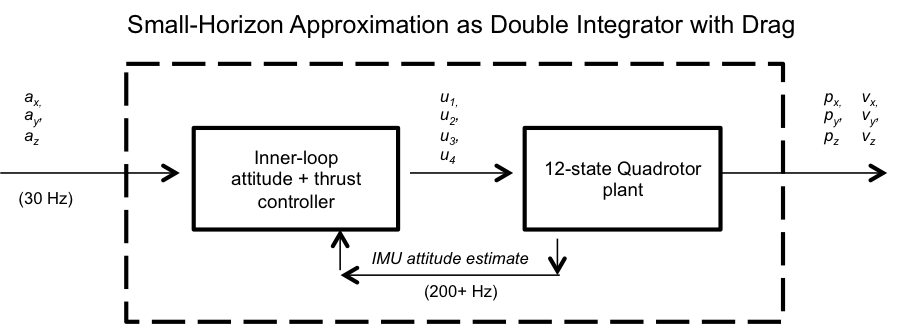
\includegraphics[width=\linewidth]{double_integrator_approximation.png}
  \caption{Dynamics approximation considered: the quadrotor is modeled in feedback with the inner loop attitude and thrust controller.}
  \label{fig:boat1}
\end{figure}

\textbf{Approach}
\\

The simple summary of this formulation is that the online control choice is the action, $\mathbb{A}_i$, that minimizes the sum of costs (where each $k$ is just a weighting factor):

$$ \underset{i}{\text{argmin}} \bigg[ k_{tg}\big[ cost(\mathbb{A}_i)_{\text{towards goal}}  \big]+  k_{s} \big[ cost(\mathbb{A}_i)_{\text{switching}} \big]+   k_{pc}\big[ cost(\mathbb{A}_i)_{\text{probabilistic collision}} \big]  \bigg]$$


Inputs required are: (i) an instantaneous depth image containing $r \times c = M$ points in relative coordinates $x_i, y_i, z_i$ and each with covariance $\Sigma_{d.r.}$, (ii) estimates for the linear $x, y, z$ velocities with covariance $\Sigma_{v_0}$, and (iii) the $x,y,z$ location of a local goal.  As a first, simple approach, the $cost(\mathbb{A}_i)_{\text{towards goal}} $ can be approximated via Euclidean distance to the local goal.\\

The actions considered live in the input space to the double integrator approximation: accelerations in $\mathbb{R}^3$.  To create the bins for $a_x$ and $a_y$ each, we approximate the maximum horizontal acceleration and sample over possible horizontal accelerations around a circle in the horizontal plane.   The max horizontal acceleration is approximated as the maximum thrust vector ($T_{max}$, easy to measure) angled just enough to compensate for gravity: $a_{max} = \frac{ \sqrt{ T_{max}^2 + (mg)^2}}{m}$.  By sampling both over the horizontal acceleration with just a few discretizations (for example, [$a_{max}, 0.6a_{max}, 0.3*a_{max} ]$) and just 8 evenly spaced $\theta$ over $[0, 2\pi]$, this yields a useful 24 options in the horizontal plane.  The figure below is a depiction of forming the horizontal $[a_x, a_y]$ bins.  For the bins where the maximum horizontal acceleration is used, we only use $a_z = 0$ since thrust is already saturated, but when thrust is not saturated we add up vertical options as well $a_z = [-a_{vert}, 0, a_{vert}]$. This makes for a total of 56 $[a_x, a_y, a_z]$ actions for the quadrotor to consider.\\

\begin{figure}
  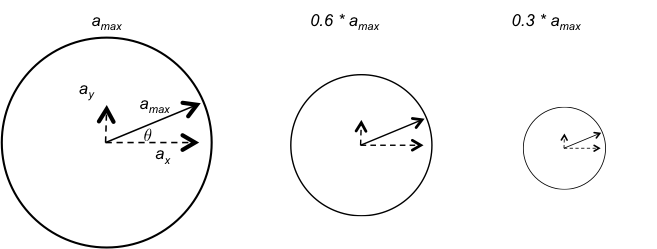
\includegraphics[width=\linewidth]{horizontal_actions.png}
  \caption{Formation of horizontal actions from sampling over thrust-scaled circles in the horizontal plane.}
  \label{fig:boat1}
\end{figure}

Over the small receding planning horizon (we use a finite time horizon $t_f = 500$ ms at least to start out), paths through configuration space can be trivially calculated at any moment, due to the simple constant-acceleration point-mass model (double integrator).  A benefit of this simple model is that due to the constant accelerations and the independence of $x, y, z$, we do not even need to sequentially forward-simulate a trajectory by integration, instead we can calculate directly the position $\mathbf{p}(t)$ of the robot for any time.  Calculating each position of each action at each time is 100\% parallelizable.

$$ \textbf{p}_i(t) = \frac{1}{2} \textbf{a}_i t^2 + \mathbf{v}_0 t \ \ \ \text{for action} \  \mathbb{A}_i$$

Note that initial positions are always considered to be $[0,0,0]$, since we are in the robot's relative coordinates.  The linear velocity estimates $\mathbf{v}_0$ coming from our state estimation system are the random variables, as will be discussed in the probabilistic collision calculations.\\

The on-line decision requires the evaluation of each of the possible actions:
$$ cost(\mathbb{A}_i)_{\text{total}} = k_{tg}\big[ cost(\mathbb{A}_i)_{\text{towards goal}}  \big]+  k_{s} \big[ cost(\mathbb{A}_i)_{\text{switching}} \big]+   k_{pc}\big[ cost(\mathbb{A}_i)_{\text{probabilistic collision}} \big] $$

The first and second terms, the costs towards the goal and the switching (stubborn) costs are trivial to evaluate.  As a first approximation we can evaluate the cost towards the goal as the Euclidean distance to the provided local goal:

$$cost(\mathbb{A}_i)_{\text{towards goal}} = || \mathbf{p}_i(t_f) - \mathbf{p}_{goal} ||_2 $$

And the cost of switching can be defined as a norm in the input space (desired accelerations) between the previous input and the considered new input.  We guess the 1-norm is reasonable:

$$cost(\mathbb{A}_i)_{\text{switching}} = || \textbf{a}_i - \textbf{a}_{previous} ||_1 $$

The probabilistic collision term is overwhelmingly the most computationally complex.  It is actually trivial, due to products of Gaussians also being Gaussians, to calculate the probability density for any (i) single action, (ii) single point in time, with (iii) a single depth return in the point cloud.  With the simple point-mass model, every single one of these computations is parallelizable.\\

For each $\mathbb{A}_i$ at each $t$, we assume that the robot's future position is a Gaussian distribution: 

$$\mathbf{p}(t) \sim N(\mathbf{\hat{p}}(t), \Sigma_p(t))$$

Where the covariance of the position is due to the appropriate scaling of the initial velocity covariance (recall $ \textbf{p}_i(t) = \frac{1}{2} \textbf{a}_i t^2 + \mathbf{v}_0 t$):

$$ \Sigma_{p_i(t)} = t^2 \Sigma_{v_0}$$

We also have a Gaussian distribution on each of the points from each of the $j$ depth returns, $\mathbf{p}_{j} \sim N(\mathbf{\hat{p}}_{j}, \Sigma_{d.r.})$.  The $\Sigma_{d.r.}$ can be approximated as uniform for each point in the point cloud, and estimated from sensor data or a sensor specification sheet.\\

It is known that the product of two Gaussian distributions is itself a Gaussian, and independence of the robot position distribution and the sensor distribution is a fair assumption, so we have for the joint distribution:

$$ p(\text{collision}_{i,j,t}) = \frac{1}{\sqrt{\text{det}}(2 \pi \Sigma_{C(i, t)})} \exp \big[  -\frac{1}{2}(\mathbf{\hat{p}}(t) - \mathbf{\hat{p}}_{j})^T \Sigma_{C(i, t)}^{-1} (\mathbf{\hat{p}}(t) - \mathbf{\hat{p}}_{j}) \big] $$

Where $\Sigma_{C(i, t)} = \Sigma_{p_i(t)} + \Sigma_{d.r.}$.  The above only gives the probability density for a given point (which is measure 0), rather than a integral of the density over some volume.  We note that in chance-constrained programming (Toit 2012), because calculating an actual probability is desired in order to pose a chance constraint, they approximate the integral with a small-sphere approximation, multiplying the volume of the robot $V_r$ by the probability density at the mean.  For us, however, since the probabilistic aspect is considered as part of the objective, the volume would just be a linear scaling for each and every probability calculated, and so it is not needed.\\

For a given (i) single action, (ii) single point in time, and (iii) a single depth return in the point cloud, the above (with a small volume approximation) could actually be considered a probability (between [0,1]).  Since we want to calculate a cost of collision for (i) a single action, but over all future time and over all possible points in the point cloud, we want a metric which includes all time and all points.  Although it is not a ``probability'' (not between [0,1]), we sum all of the individual probabilities for a given action:

$$cost(\mathbb{A}_i)_{\text{probabilistic collision}} = \sum_j \sum_t p(\text{collision}_{i,j,t}) $$

Which can be thought of as an un-normalized (linear scaling doesn't matter) weighted average of the probability of collision.

We now consider the complexity of this naive algorithm.  The complexity grows naively as:

$$\text{Naive complexity:} \ \ \ O( n_{A} \times n_{t.s.} \times n_{j})$$

Where $n_A$ is the number of actions (~50 is sufficient), $n_{t.s.}$ is the number of time steps considered linearly between $[0, t_f]$ (~20 is sufficient), and $n_{j}$ is the number of depth returns, which is by far the largest.  Even for a ``low-resolution'' 160x120 depth image, this worst-case is $M=19,200$ points (it is not as bad of no-returns are provided for most of the pixels).\\

As an approach to significantly reduce complexity of probabilistic collision cost, the depth returns can be processed once into a $k$-$d$-tree, and then efficient evaluation can be to look up the closest depth returns for each $\mathbf{p}_i(t)$.  Only the closest $n_j \approx 10$ depth returns, for example, could be used to calculate the probabilistic collision cost.\\

Once the lowest-cost action is selected, it can be executed ``open-loop'' for only 30 Hz, until the next depth image is available.  A generalization could allow ``open-loop'' $u$-tapes to happen for 30 Hz, rather than just one $u$.  The ``outer-loop'' of this fast MPC-type framework keeps the quadrotor heading towards the right direction safely.\\

\textbf{Alternative using a local map}
\\

It is useful to consider that rather than introducing a stubborn cost (which is a very simple encoding of previous depth information / hysteresis), another approach could include a local map.\\

Rather than only consider the instantaneous depth image, the last $N$ depth images could be used, and each time a depth image + state estimate is received, a $k$-$d$-tree that holds $N \times M$ points could be used.  The variances of the older depth image points would ``grow'' considerably over time in our model, becoming blurry compared to the fresh depth returns.  \\

\textbf{To do}
\\
\begin{itemize}
\item Finish simple sim implementation (working on now)
\item Add drag to dynamics approximation (easy)
\item Consider constant-jerk formulation
\item Figure out how to handle trajectories going outside field of view (FOV) -- a simple option is to just not consider them.  But if you 100\% see a wall in front of you, you are better off venturing into a blind spot.  Unknown is worse than known unoccupied, but not as bad as known occupied.
\item Limit velocity based on some high-level input (this is easy, just discard any trajectories with terminal velocities above the higher-level limit)
\end{itemize}










%----------------------------------------------------------------------------------------

\end{document}